% Created by tikzDevice version 0.10.1 on 2016-09-02 18:57:15
% !TEX encoding = UTF-8 Unicode
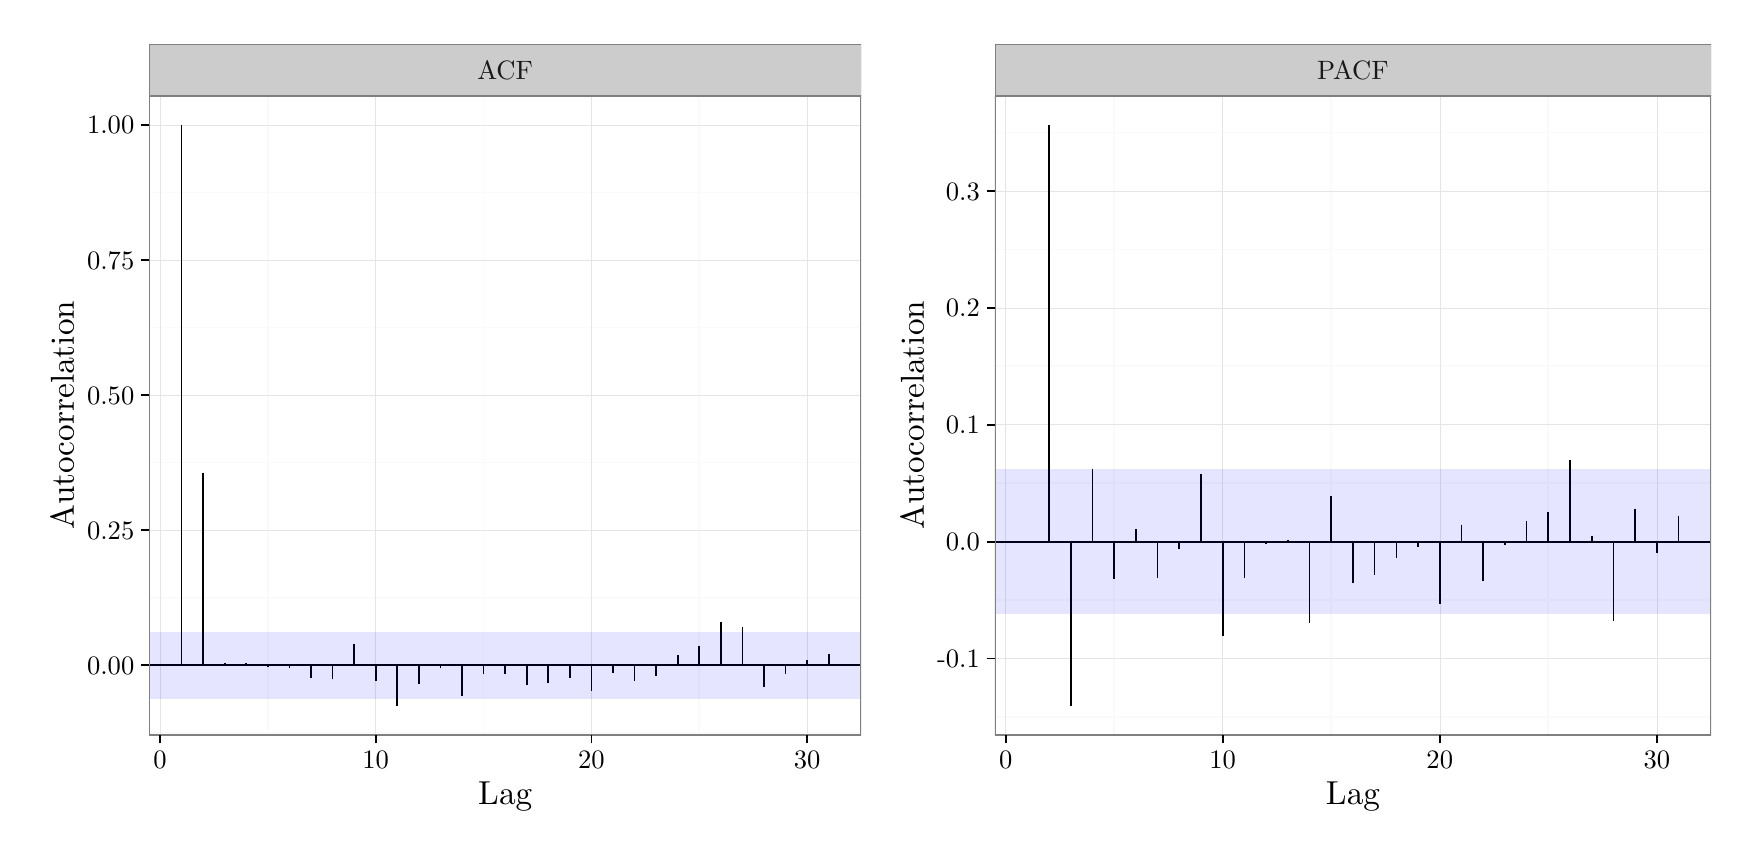
\begin{tikzpicture}[x=1pt,y=1pt]
\definecolor{fillColor}{RGB}{255,255,255}
\path[use as bounding box,fill=fillColor,fill opacity=0.00] (0,0) rectangle (614.29,289.08);
\begin{scope}
\path[clip] (  0.00,  0.00) rectangle (307.15,289.08);
\definecolor{drawColor}{RGB}{255,255,255}
\definecolor{fillColor}{RGB}{255,255,255}

\path[draw=drawColor,line width= 0.6pt,line join=round,line cap=round,fill=fillColor] ( -0.00,  0.00) rectangle (307.15,289.08);
\end{scope}
\begin{scope}
\path[clip] ( 43.93, 33.48) rectangle (301.15,264.47);
\definecolor{fillColor}{RGB}{255,255,255}

\path[fill=fillColor] ( 43.93, 33.48) rectangle (301.15,264.47);
\definecolor{drawColor}{gray}{0.98}

\path[draw=drawColor,line width= 0.6pt,line join=round] ( 43.93, 34.26) --
	(301.15, 34.26);

\path[draw=drawColor,line width= 0.6pt,line join=round] ( 43.93, 83.09) --
	(301.15, 83.09);

\path[draw=drawColor,line width= 0.6pt,line join=round] ( 43.93,131.91) --
	(301.15,131.91);

\path[draw=drawColor,line width= 0.6pt,line join=round] ( 43.93,180.73) --
	(301.15,180.73);

\path[draw=drawColor,line width= 0.6pt,line join=round] ( 43.93,229.56) --
	(301.15,229.56);

\path[draw=drawColor,line width= 0.6pt,line join=round] ( 86.80, 33.48) --
	( 86.80,264.47);

\path[draw=drawColor,line width= 0.6pt,line join=round] (164.74, 33.48) --
	(164.74,264.47);

\path[draw=drawColor,line width= 0.6pt,line join=round] (242.69, 33.48) --
	(242.69,264.47);
\definecolor{drawColor}{gray}{0.90}

\path[draw=drawColor,line width= 0.2pt,line join=round] ( 43.93, 58.68) --
	(301.15, 58.68);

\path[draw=drawColor,line width= 0.2pt,line join=round] ( 43.93,107.50) --
	(301.15,107.50);

\path[draw=drawColor,line width= 0.2pt,line join=round] ( 43.93,156.32) --
	(301.15,156.32);

\path[draw=drawColor,line width= 0.2pt,line join=round] ( 43.93,205.15) --
	(301.15,205.15);

\path[draw=drawColor,line width= 0.2pt,line join=round] ( 43.93,253.97) --
	(301.15,253.97);

\path[draw=drawColor,line width= 0.2pt,line join=round] ( 47.82, 33.48) --
	( 47.82,264.47);

\path[draw=drawColor,line width= 0.2pt,line join=round] (125.77, 33.48) --
	(125.77,264.47);

\path[draw=drawColor,line width= 0.2pt,line join=round] (203.72, 33.48) --
	(203.72,264.47);

\path[draw=drawColor,line width= 0.2pt,line join=round] (281.66, 33.48) --
	(281.66,264.47);
\definecolor{drawColor}{RGB}{0,0,0}

\path[draw=drawColor,line width= 0.6pt,line join=round] ( 43.93, 58.68) -- (301.15, 58.68);

\path[draw=drawColor,line width= 0.6pt,line join=round] ( 55.62,253.97) -- ( 55.62, 58.68);

\path[draw=drawColor,line width= 0.6pt,line join=round] ( 63.41,128.29) -- ( 63.41, 58.68);

\path[draw=drawColor,line width= 0.6pt,line join=round] ( 71.21, 59.55) -- ( 71.21, 58.68);

\path[draw=drawColor,line width= 0.6pt,line join=round] ( 79.00, 59.63) -- ( 79.00, 58.68);

\path[draw=drawColor,line width= 0.6pt,line join=round] ( 86.80, 57.92) -- ( 86.80, 58.68);

\path[draw=drawColor,line width= 0.6pt,line join=round] ( 94.59, 57.81) -- ( 94.59, 58.68);

\path[draw=drawColor,line width= 0.6pt,line join=round] (102.39, 54.12) -- (102.39, 58.68);

\path[draw=drawColor,line width= 0.6pt,line join=round] (110.18, 53.62) -- (110.18, 58.68);

\path[draw=drawColor,line width= 0.6pt,line join=round] (117.98, 66.44) -- (117.98, 58.68);

\path[draw=drawColor,line width= 0.6pt,line join=round] (125.77, 53.06) -- (125.77, 58.68);

\path[draw=drawColor,line width= 0.6pt,line join=round] (133.56, 43.98) -- (133.56, 58.68);

\path[draw=drawColor,line width= 0.6pt,line join=round] (141.36, 51.74) -- (141.36, 58.68);

\path[draw=drawColor,line width= 0.6pt,line join=round] (149.15, 57.60) -- (149.15, 58.68);

\path[draw=drawColor,line width= 0.6pt,line join=round] (156.95, 47.54) -- (156.95, 58.68);

\path[draw=drawColor,line width= 0.6pt,line join=round] (164.74, 55.55) -- (164.74, 58.68);

\path[draw=drawColor,line width= 0.6pt,line join=round] (172.54, 55.70) -- (172.54, 58.68);

\path[draw=drawColor,line width= 0.6pt,line join=round] (180.33, 51.57) -- (180.33, 58.68);

\path[draw=drawColor,line width= 0.6pt,line join=round] (188.13, 52.16) -- (188.13, 58.68);

\path[draw=drawColor,line width= 0.6pt,line join=round] (195.92, 54.24) -- (195.92, 58.68);

\path[draw=drawColor,line width= 0.6pt,line join=round] (203.72, 49.36) -- (203.72, 58.68);

\path[draw=drawColor,line width= 0.6pt,line join=round] (211.51, 55.90) -- (211.51, 58.68);

\path[draw=drawColor,line width= 0.6pt,line join=round] (219.30, 53.13) -- (219.30, 58.68);

\path[draw=drawColor,line width= 0.6pt,line join=round] (227.10, 54.88) -- (227.10, 58.68);

\path[draw=drawColor,line width= 0.6pt,line join=round] (234.89, 62.34) -- (234.89, 58.68);

\path[draw=drawColor,line width= 0.6pt,line join=round] (242.69, 65.79) -- (242.69, 58.68);

\path[draw=drawColor,line width= 0.6pt,line join=round] (250.48, 74.41) -- (250.48, 58.68);

\path[draw=drawColor,line width= 0.6pt,line join=round] (258.28, 72.56) -- (258.28, 58.68);

\path[draw=drawColor,line width= 0.6pt,line join=round] (266.07, 50.99) -- (266.07, 58.68);

\path[draw=drawColor,line width= 0.6pt,line join=round] (273.87, 55.57) -- (273.87, 58.68);

\path[draw=drawColor,line width= 0.6pt,line join=round] (281.66, 60.48) -- (281.66, 58.68);

\path[draw=drawColor,line width= 0.6pt,line join=round] (289.46, 62.59) -- (289.46, 58.68);
\definecolor{fillColor}{RGB}{0,0,255}

\path[fill=fillColor,fill opacity=0.10] ( 43.93, 46.57) rectangle (301.15, 70.78);
\definecolor{drawColor}{gray}{0.50}

\path[draw=drawColor,line width= 0.6pt,line join=round,line cap=round] ( 43.93, 33.48) rectangle (301.15,264.47);
\end{scope}
\begin{scope}
\path[clip] ( 43.93,264.47) rectangle (301.15,283.08);
\definecolor{drawColor}{gray}{0.50}
\definecolor{fillColor}{gray}{0.80}

\path[draw=drawColor,line width= 0.2pt,line join=round,line cap=round,fill=fillColor] ( 43.93,264.47) rectangle (301.15,283.08);
\definecolor{drawColor}{gray}{0.10}

\node[text=drawColor,anchor=base,inner sep=0pt, outer sep=0pt, scale=  0.96] at (172.54,270.47) {ACF};
\end{scope}
\begin{scope}
\path[clip] (  0.00,  0.00) rectangle (614.29,289.08);
\definecolor{drawColor}{RGB}{0,0,0}

\node[text=drawColor,anchor=base east,inner sep=0pt, outer sep=0pt, scale=  0.96] at ( 38.53, 55.37) {0.00};

\node[text=drawColor,anchor=base east,inner sep=0pt, outer sep=0pt, scale=  0.96] at ( 38.53,104.19) {0.25};

\node[text=drawColor,anchor=base east,inner sep=0pt, outer sep=0pt, scale=  0.96] at ( 38.53,153.02) {0.50};

\node[text=drawColor,anchor=base east,inner sep=0pt, outer sep=0pt, scale=  0.96] at ( 38.53,201.84) {0.75};

\node[text=drawColor,anchor=base east,inner sep=0pt, outer sep=0pt, scale=  0.96] at ( 38.53,250.66) {1.00};
\end{scope}
\begin{scope}
\path[clip] (  0.00,  0.00) rectangle (614.29,289.08);
\definecolor{drawColor}{RGB}{0,0,0}

\path[draw=drawColor,line width= 0.6pt,line join=round] ( 40.93, 58.68) --
	( 43.93, 58.68);

\path[draw=drawColor,line width= 0.6pt,line join=round] ( 40.93,107.50) --
	( 43.93,107.50);

\path[draw=drawColor,line width= 0.6pt,line join=round] ( 40.93,156.32) --
	( 43.93,156.32);

\path[draw=drawColor,line width= 0.6pt,line join=round] ( 40.93,205.15) --
	( 43.93,205.15);

\path[draw=drawColor,line width= 0.6pt,line join=round] ( 40.93,253.97) --
	( 43.93,253.97);
\end{scope}
\begin{scope}
\path[clip] (  0.00,  0.00) rectangle (614.29,289.08);
\definecolor{drawColor}{RGB}{0,0,0}

\path[draw=drawColor,line width= 0.6pt,line join=round] ( 47.82, 30.48) --
	( 47.82, 33.48);

\path[draw=drawColor,line width= 0.6pt,line join=round] (125.77, 30.48) --
	(125.77, 33.48);

\path[draw=drawColor,line width= 0.6pt,line join=round] (203.72, 30.48) --
	(203.72, 33.48);

\path[draw=drawColor,line width= 0.6pt,line join=round] (281.66, 30.48) --
	(281.66, 33.48);
\end{scope}
\begin{scope}
\path[clip] (  0.00,  0.00) rectangle (614.29,289.08);
\definecolor{drawColor}{RGB}{0,0,0}

\node[text=drawColor,anchor=base,inner sep=0pt, outer sep=0pt, scale=  0.96] at ( 47.82, 21.46) {0};

\node[text=drawColor,anchor=base,inner sep=0pt, outer sep=0pt, scale=  0.96] at (125.77, 21.46) {10};

\node[text=drawColor,anchor=base,inner sep=0pt, outer sep=0pt, scale=  0.96] at (203.72, 21.46) {20};

\node[text=drawColor,anchor=base,inner sep=0pt, outer sep=0pt, scale=  0.96] at (281.66, 21.46) {30};
\end{scope}
\begin{scope}
\path[clip] (  0.00,  0.00) rectangle (614.29,289.08);
\definecolor{drawColor}{RGB}{0,0,0}

\node[text=drawColor,anchor=base,inner sep=0pt, outer sep=0pt, scale=  1.20] at (172.54,  8.40) {Lag};
\end{scope}
\begin{scope}
\path[clip] (  0.00,  0.00) rectangle (614.29,289.08);
\definecolor{drawColor}{RGB}{0,0,0}

\node[text=drawColor,rotate= 90.00,anchor=base,inner sep=0pt, outer sep=0pt, scale=  1.20] at ( 16.66,148.97) {Autocorrelation};
\end{scope}
\begin{scope}
\path[clip] (307.15,  0.00) rectangle (614.29,289.08);
\definecolor{drawColor}{RGB}{255,255,255}
\definecolor{fillColor}{RGB}{255,255,255}

\path[draw=drawColor,line width= 0.6pt,line join=round,line cap=round,fill=fillColor] (307.15,  0.00) rectangle (614.29,289.08);
\end{scope}
\begin{scope}
\path[clip] (349.48, 33.48) rectangle (608.30,264.47);
\definecolor{fillColor}{RGB}{255,255,255}

\path[fill=fillColor] (349.48, 33.48) rectangle (608.29,264.47);
\definecolor{drawColor}{gray}{0.98}

\path[draw=drawColor,line width= 0.6pt,line join=round] (349.48, 39.95) --
	(608.30, 39.95);

\path[draw=drawColor,line width= 0.6pt,line join=round] (349.48, 82.20) --
	(608.30, 82.20);

\path[draw=drawColor,line width= 0.6pt,line join=round] (349.48,124.46) --
	(608.30,124.46);

\path[draw=drawColor,line width= 0.6pt,line join=round] (349.48,166.72) --
	(608.30,166.72);

\path[draw=drawColor,line width= 0.6pt,line join=round] (349.48,208.98) --
	(608.30,208.98);

\path[draw=drawColor,line width= 0.6pt,line join=round] (349.48,251.23) --
	(608.30,251.23);

\path[draw=drawColor,line width= 0.6pt,line join=round] (392.61, 33.48) --
	(392.61,264.47);

\path[draw=drawColor,line width= 0.6pt,line join=round] (471.04, 33.48) --
	(471.04,264.47);

\path[draw=drawColor,line width= 0.6pt,line join=round] (549.47, 33.48) --
	(549.47,264.47);
\definecolor{drawColor}{gray}{0.90}

\path[draw=drawColor,line width= 0.2pt,line join=round] (349.48, 61.08) --
	(608.30, 61.08);

\path[draw=drawColor,line width= 0.2pt,line join=round] (349.48,103.33) --
	(608.30,103.33);

\path[draw=drawColor,line width= 0.2pt,line join=round] (349.48,145.59) --
	(608.30,145.59);

\path[draw=drawColor,line width= 0.2pt,line join=round] (349.48,187.85) --
	(608.30,187.85);

\path[draw=drawColor,line width= 0.2pt,line join=round] (349.48,230.11) --
	(608.30,230.11);

\path[draw=drawColor,line width= 0.2pt,line join=round] (353.40, 33.48) --
	(353.40,264.47);

\path[draw=drawColor,line width= 0.2pt,line join=round] (431.83, 33.48) --
	(431.83,264.47);

\path[draw=drawColor,line width= 0.2pt,line join=round] (510.26, 33.48) --
	(510.26,264.47);

\path[draw=drawColor,line width= 0.2pt,line join=round] (588.69, 33.48) --
	(588.69,264.47);
\definecolor{drawColor}{RGB}{0,0,0}

\path[draw=drawColor,line width= 0.6pt,line join=round] (349.48,103.33) -- (608.30,103.33);

\path[draw=drawColor,line width= 0.6pt,line join=round] (369.08,253.97) -- (369.08,103.33);

\path[draw=drawColor,line width= 0.6pt,line join=round] (376.93, 43.98) -- (376.93,103.33);

\path[draw=drawColor,line width= 0.6pt,line join=round] (384.77,129.57) -- (384.77,103.33);

\path[draw=drawColor,line width= 0.6pt,line join=round] (392.61, 89.80) -- (392.61,103.33);

\path[draw=drawColor,line width= 0.6pt,line join=round] (400.45,107.85) -- (400.45,103.33);

\path[draw=drawColor,line width= 0.6pt,line join=round] (408.30, 90.35) -- (408.30,103.33);

\path[draw=drawColor,line width= 0.6pt,line join=round] (416.14,100.57) -- (416.14,103.33);

\path[draw=drawColor,line width= 0.6pt,line join=round] (423.98,127.71) -- (423.98,103.33);

\path[draw=drawColor,line width= 0.6pt,line join=round] (431.83, 69.22) -- (431.83,103.33);

\path[draw=drawColor,line width= 0.6pt,line join=round] (439.67, 90.04) -- (439.67,103.33);

\path[draw=drawColor,line width= 0.6pt,line join=round] (447.51,102.57) -- (447.51,103.33);

\path[draw=drawColor,line width= 0.6pt,line join=round] (455.36,104.11) -- (455.36,103.33);

\path[draw=drawColor,line width= 0.6pt,line join=round] (463.20, 73.97) -- (463.20,103.33);

\path[draw=drawColor,line width= 0.6pt,line join=round] (471.04,119.90) -- (471.04,103.33);

\path[draw=drawColor,line width= 0.6pt,line join=round] (478.89, 88.27) -- (478.89,103.33);

\path[draw=drawColor,line width= 0.6pt,line join=round] (486.73, 91.46) -- (486.73,103.33);

\path[draw=drawColor,line width= 0.6pt,line join=round] (494.57, 97.58) -- (494.57,103.33);

\path[draw=drawColor,line width= 0.6pt,line join=round] (502.41,101.34) -- (502.41,103.33);

\path[draw=drawColor,line width= 0.6pt,line join=round] (510.26, 80.84) -- (510.26,103.33);

\path[draw=drawColor,line width= 0.6pt,line join=round] (518.10,109.49) -- (518.10,103.33);

\path[draw=drawColor,line width= 0.6pt,line join=round] (525.94, 89.15) -- (525.94,103.33);

\path[draw=drawColor,line width= 0.6pt,line join=round] (533.79,101.99) -- (533.79,103.33);

\path[draw=drawColor,line width= 0.6pt,line join=round] (541.63,110.87) -- (541.63,103.33);

\path[draw=drawColor,line width= 0.6pt,line join=round] (549.47,113.97) -- (549.47,103.33);

\path[draw=drawColor,line width= 0.6pt,line join=round] (557.32,132.82) -- (557.32,103.33);

\path[draw=drawColor,line width= 0.6pt,line join=round] (565.16,105.49) -- (565.16,103.33);

\path[draw=drawColor,line width= 0.6pt,line join=round] (573.00, 74.68) -- (573.00,103.33);

\path[draw=drawColor,line width= 0.6pt,line join=round] (580.84,115.30) -- (580.84,103.33);

\path[draw=drawColor,line width= 0.6pt,line join=round] (588.69, 99.33) -- (588.69,103.33);

\path[draw=drawColor,line width= 0.6pt,line join=round] (596.53,112.80) -- (596.53,103.33);
\definecolor{fillColor}{RGB}{0,0,255}

\path[fill=fillColor,fill opacity=0.10] (349.48, 77.14) rectangle (608.29,129.52);
\definecolor{drawColor}{gray}{0.50}

\path[draw=drawColor,line width= 0.6pt,line join=round,line cap=round] (349.48, 33.48) rectangle (608.29,264.47);
\end{scope}
\begin{scope}
\path[clip] (349.48,264.47) rectangle (608.30,283.08);
\definecolor{drawColor}{gray}{0.50}
\definecolor{fillColor}{gray}{0.80}

\path[draw=drawColor,line width= 0.2pt,line join=round,line cap=round,fill=fillColor] (349.48,264.47) rectangle (608.29,283.08);
\definecolor{drawColor}{gray}{0.10}

\node[text=drawColor,anchor=base,inner sep=0pt, outer sep=0pt, scale=  0.96] at (478.89,270.47) {PACF};
\end{scope}
\begin{scope}
\path[clip] (  0.00,  0.00) rectangle (614.29,289.08);
\definecolor{drawColor}{RGB}{0,0,0}

\node[text=drawColor,anchor=base east,inner sep=0pt, outer sep=0pt, scale=  0.96] at (344.08, 57.77) {-0.1};

\node[text=drawColor,anchor=base east,inner sep=0pt, outer sep=0pt, scale=  0.96] at (344.08,100.03) {0.0};

\node[text=drawColor,anchor=base east,inner sep=0pt, outer sep=0pt, scale=  0.96] at (344.08,142.29) {0.1};

\node[text=drawColor,anchor=base east,inner sep=0pt, outer sep=0pt, scale=  0.96] at (344.08,184.54) {0.2};

\node[text=drawColor,anchor=base east,inner sep=0pt, outer sep=0pt, scale=  0.96] at (344.08,226.80) {0.3};
\end{scope}
\begin{scope}
\path[clip] (  0.00,  0.00) rectangle (614.29,289.08);
\definecolor{drawColor}{RGB}{0,0,0}

\path[draw=drawColor,line width= 0.6pt,line join=round] (346.48, 61.08) --
	(349.48, 61.08);

\path[draw=drawColor,line width= 0.6pt,line join=round] (346.48,103.33) --
	(349.48,103.33);

\path[draw=drawColor,line width= 0.6pt,line join=round] (346.48,145.59) --
	(349.48,145.59);

\path[draw=drawColor,line width= 0.6pt,line join=round] (346.48,187.85) --
	(349.48,187.85);

\path[draw=drawColor,line width= 0.6pt,line join=round] (346.48,230.11) --
	(349.48,230.11);
\end{scope}
\begin{scope}
\path[clip] (  0.00,  0.00) rectangle (614.29,289.08);
\definecolor{drawColor}{RGB}{0,0,0}

\path[draw=drawColor,line width= 0.6pt,line join=round] (353.40, 30.48) --
	(353.40, 33.48);

\path[draw=drawColor,line width= 0.6pt,line join=round] (431.83, 30.48) --
	(431.83, 33.48);

\path[draw=drawColor,line width= 0.6pt,line join=round] (510.26, 30.48) --
	(510.26, 33.48);

\path[draw=drawColor,line width= 0.6pt,line join=round] (588.69, 30.48) --
	(588.69, 33.48);
\end{scope}
\begin{scope}
\path[clip] (  0.00,  0.00) rectangle (614.29,289.08);
\definecolor{drawColor}{RGB}{0,0,0}

\node[text=drawColor,anchor=base,inner sep=0pt, outer sep=0pt, scale=  0.96] at (353.40, 21.46) {0};

\node[text=drawColor,anchor=base,inner sep=0pt, outer sep=0pt, scale=  0.96] at (431.83, 21.46) {10};

\node[text=drawColor,anchor=base,inner sep=0pt, outer sep=0pt, scale=  0.96] at (510.26, 21.46) {20};

\node[text=drawColor,anchor=base,inner sep=0pt, outer sep=0pt, scale=  0.96] at (588.69, 21.46) {30};
\end{scope}
\begin{scope}
\path[clip] (  0.00,  0.00) rectangle (614.29,289.08);
\definecolor{drawColor}{RGB}{0,0,0}

\node[text=drawColor,anchor=base,inner sep=0pt, outer sep=0pt, scale=  1.20] at (478.89,  8.40) {Lag};
\end{scope}
\begin{scope}
\path[clip] (  0.00,  0.00) rectangle (614.29,289.08);
\definecolor{drawColor}{RGB}{0,0,0}

\node[text=drawColor,rotate= 90.00,anchor=base,inner sep=0pt, outer sep=0pt, scale=  1.20] at (323.81,148.97) {Autocorrelation};
\end{scope}
\end{tikzpicture}
